\documentclass[tikz, border=10pt]{standalone}

\usepackage{tikz}

\begin{document}

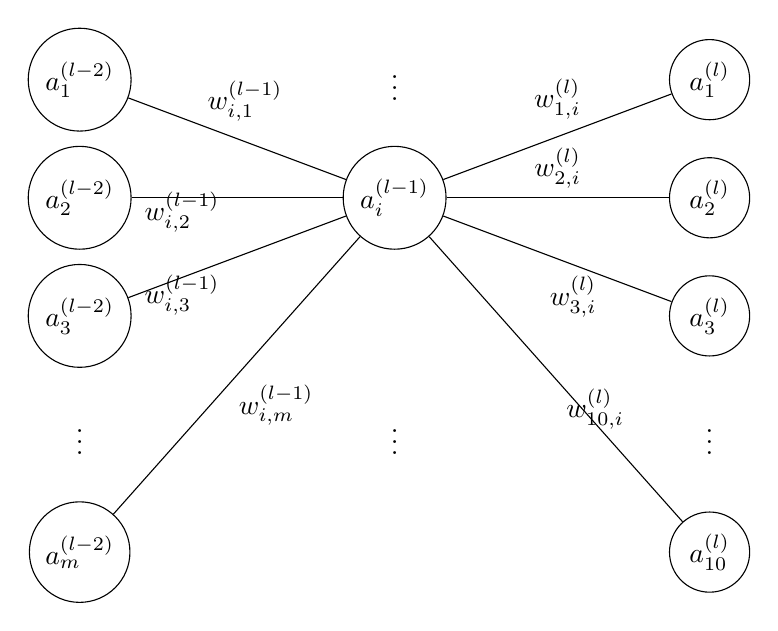
\begin{tikzpicture}[
    neuron/.style={circle, draw, minimum size=1cm}
]

    % l-2 layer
    \foreach \i in {1,...,3}
        \node[neuron] (L_2\i) at (0,-\i*1.5) {$a_{\i}^{(l-2)}$};

    \node at (0, {-4*1.5}) {\vdots};

    \node[neuron] (L_24) at (0,-5*1.5) {$a_{m}^{(l-2)}$};

    % l-1 layer

    \node at (4, -1.5) {\vdots};

    \node[neuron] (L_1) at (4, -3) {$a_{i}^{(l-1)}$};

    \node at (4, {-4*1.5}) {\vdots};

    % l layer
    \foreach \i in {1,...,3}
        \node[neuron] (O\i) at (8,-\i*1.5) {$a_{\i}^{(l)}$};

    \node at (8, {-4*1.5}) {\vdots};

    \node[neuron] (O4) at (8,-5*1.5) {$a_{10}^{(l)}$};

    \draw (L_1) --node[midway, above, yshift=0.1cm] {$w_{1,i}^{(l)}$} (O1);
    \draw (L_1) --node[midway, above] {$w_{2,i}^{(l)}$} (O2);
    \draw (L_1) --node[midway, below, xshift=0.2cm, yshift=-0.1cm] {$w_{3,i}^{(l)}$} (O3);
    \draw (L_1) --node[midway, below, xshift=0.5cm] {$w_{10,i}^{(l)}$} (O4);

    \draw (L_21) --node[midway, above, xshift=0.1cm, yshift=0.1cm] {$w_{i,1}^{(l-1)}$} (L_1);
    \draw (L_22) --node[midway, below, xshift=-0.7cm, yshift=0.2cm] {$w_{i,2}^{(l-1)}$} (L_1);
    \draw (L_23) --node[midway, below, xshift=-0.7cm, yshift=-0.1cm] {$w_{i,3}^{(l-1)}$} (L_1);
    \draw (L_24) --node[midway, below, xshift=0.5cm] {$w_{i,m}^{(l-1)}$} (L_1);


\end{tikzpicture}

\end{document}
